\section{History}

This package was born out of a $\approx$~10 line function I wrote to estimate the memory usage of (non-allocated) in-core, dense \proglang{R} objects of numeric (double precision) data.  I need this in my life by a surprising amount, so it made sense to actually create this thing instead of constantly doing ad hoc multiplications of $nrows\times ncols \times 8$ then dividing by powers of $1024$ (or 1000).

But then I got the great idea to make this application $\sim$~\hspace{-.1cm}enterprise ready\hspace{-.1cm}~$\sim$ by adding a lot of unnecessary and convoluted OOP, and this stupid package was born.  This is sort of a love letter to other needlessly complex programs, like the \href{https://github.com/Mikkeren/FizzBuzzEnterpriseEdition}{Enterprise Fizzbuzz}\footnote{If you are unfamiliar with the \href{https://en.wikipedia.org/wiki/Bizz_buzz}{fizzbuzz}, see my posts ``\href{http://librestats.com/2012/01/10/honing-your-r-skills-for-job-interviews/}{Honing your R skills for Job Interviews}'' and ``\href{http://librestats.com/2013/04/26/the-fizzbuzz-that-fortran-deserves/}{The Fizzbuzz that Fortran Deserves}''.}.



\section{License}

\begin{figure}[th]
  \centering
  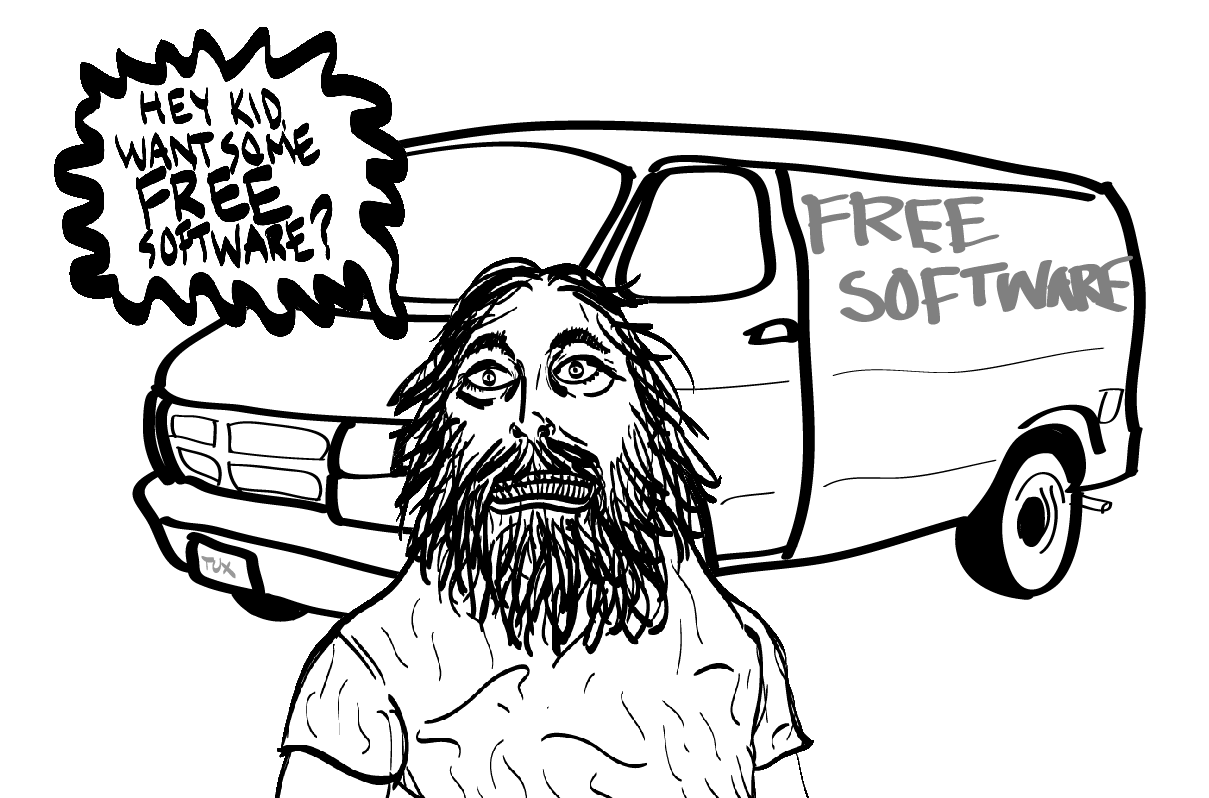
\includegraphics[scale=.35]{./include/gpl.png}
  \caption{The GNU GPL Explained}
  \label{fig:gnu}
\end{figure}
This package is free software licensed under the GNU General Public License, version $\geq$ 2 (see Figure~\ref{fig:gnu}).
If you violate the terms of the GPL then Richard Stallman's beard will sue you in internet court.



\section{Installation}

The package consists entirely of \proglang{R} code, so everything should install fine no matter which platform you use.  To install this from source on Windows, you will need to first install the \href{http://cran.r-project.org/bin/windows/Rtools/Rtools216.exe}{Rtools} package.  The package should install on Mac or Linux\footnote{\interject} without problem.

The easiest way to install \pkg{MemUse} is via the \href{http://cran.r-project.org/web/packages/devtools/index.html}{\pkg{devtools}} package.  With this, you can effectively install packages from github just as you would from the CRAN.  To install \pkg{MemUse} using \pkg{devtools}, simply issue the command:
\begin{lstlisting}[language=rr]
library(devtools)
install_github(repo="memuse", username="wrathematics")
\end{lstlisting}
from R.  Alternatively, you could download the sourcecode \href{https://github.com/wrathematics/memuse/archive/master.zip}{from github}, unzip this archive, and issue the command:
\begin{lstlisting}[language=sh]
R CMD INSTALL memuse-master
\end{lstlisting}
from your shell.




\section{Using the MemUse Package}

\subsection{Size Matters, and How You Are Using It is Wrong}
The core of the \pkg{MemUse} package is the \code{memuse} class object.  You can construct a \code{memuse} object via the \code{memuse()} or \code{mu()} constructor.  The constructor has several options.  You can pass the size of the object, the unit, the unit prefix (IEC or SI), and the unit names (short or long).  The size is the number of bytes, scaled by some factor depending on the unit.  The unit is an abstract rescaling unit, like percent, used for the sake of simple comprehension at larger scales; for example, kilobyte and kibibyte are the typical storage units to represent ``roughly a thousand'' bytes (more on this later).  Finally, the unit names are for printing, i.e., controlling whether the long version (e.g., kilobyte) or short version (kB) is used.
\begin{table}[ht]
  \centering
  \begin{tabular}{|lll|lll|}\hline
    \multicolumn{3}{|c}{IEC Prefix} & \multicolumn{3}{|c|}{SI Prefix} \\\hline
    Short & Long & Factor & Short & Long & Factor\\\hline
    b & byte & 1 & b & byte & 1\\
    KiB & kibibyte & $2^{10}$ & kB & kilobyte & $10^3$\\
    MiB & mebibyte & $2^{20}$ & MB & megabyte & $10^6$\\
    GiB & gibibyte & $2^{30}$ & GB & gigabyte & $10^9$\\
    TiB & tebibyte & $2^{40}$ & TB & terabyte & $10^{12}$\\
    PiB & pebibyte & $2^{50}$ & PB & petabyte & $10^{15}$\\
    EiB & exbibyte & $2^{60}$ & EB & exabyte & $10^{18}$\\
    ZiB & zebibyte & $2^{70}$ & ZB & zettabyte & $10^{21}$\\
    YiB & yobibyte & $2^{80}$ & YB & yottabyte & $10^{24}$\\\hline
  \end{tabular}
  \caption{Units, Unit Prefices, and Scaling Factors for Byte Storage}
  \label{tab:units}
\end{table}
Table~\ref{tab:units} gives a complete list of the different units for the different prefices.

The reason for this odd distinction is that there is general ambiguity in the public versus technical definition of these terms.  People, even those who know the difference (myself included) almost overwhelmingly use, for example, gigabyte when they mean gibibyte.  The reason for this is obvious; ``gibibyte'' sounds fucking stupid.  This actually gets all the more confusing because in addition to conflating 1 MB with 1 MiB, ISP's advertise their speeds in terms of bits\footnote{1 byte is 8 bits} \emph{using the same goddamn symbol}, because they're huge assholes.

Another example is when people talk about $\sim$~\hspace{-.1cm}big data\hspace{-.1cm}~$\sim$.  Often I/O people will use the term ``terabytes'' or ``exabytes'' and mean it.  Rescaling these units into the ones people are generally more familiar with is simple with the \code{MemUse} package:
\begin{lstlisting}[language=rr]
> swap.prefix(mu(size=1, unit="tb", unit.prefix="SI"))
0.909 TiB
> swap.prefix(mu(size=1, unit="pb", unit.prefix="SI"))
0.888 PiB
\end{lstlisting}

These sizes represent an impressive amount of data, but this ambiguity in naming conventions allows people to lie a bit.  For all of these reasons, since the package is meant to be useful for understanding R object size, the default behavior is somewhat complicated, but can be summarized as trying to provide what most people meant in the first place.  We achieve this by offering several default string objects which the user can easily control.  These units are \code{.UNIT}, \code{.PREFIX}, and \code{.NAMES}.  



\subsection{Default Parameters}

The \code{.UNIT} object defaults to \code{best} and should probably just be left alone.  Functions that need to know an input unit, such as the constructor, have default argument \code{unit=.UNIT}.  Realistically, you are probably better off modifying that argument as necessary than changing \code{.UNIT}.  For example, you want to construct a 100 KiB \code{memuse} object, you probably just want to call
\begin{lstlisting}[language=rr]
mu(100, "KiB")
\end{lstlisting}
This is equivalent to calling
\begin{lstlisting}[language=rr]
mu(102400)
\end{lstlisting}
since the default \code{.UNIT=best} will make the choice to switch the units from b to KiB once you breach 1024 bytes.  This sounds a lot more confusing than it really is.

More useful is the \code{.PREFIX} parameter.  This must either be \code{SI} or \code{IEC}, with the latter being the package default.  
\begin{lstlisting}[language=rr]
> .PREFIX <- "SI"
> x <- mu(10, "kb")
> x
10.000 KB
> swap.prefix(x)
9.766 KiB
\end{lstlisting}



\subsection{Methods}
Aside from the constructor, you have already seen one very useful method:  \code{swap.prefix()}.  In addition to these, we have several other obvious methods, such as \code{swap.unit()}, \code{swap.names()}, \code{print()}, \code{show()}, etc.  But we also have some simple arithmetic, namely \code{`+`} (addition), \code{`*`} (multiplication), and \code{`\^{}`} (exponentiation).  So for example:
\begin{lstlisting}[language=rr]
> mu(100) + mu(200)
300.000 B
> mu(100) * mu(200) # 100*200/1024
19.531 KiB
\end{lstlisting}
It's not hard to implement other things like division, but I didn't because I thought it was stupid.

Finally, we have the methods that inspired the creation of this entire dumb thing in the first place:  \code{howbig()} and \code{howmany()}.  The former takes in the dimensions of a matrix (\code{nrow} rows and \code{ncol} columns) and returns the memory usage (as the package namesake would imply) of the object.  So for example, if you wanted to perform a principal components decomposition on a 100,000 by 100,000 matrix via SVD (as we have), then you would need:
\begin{lstlisting}
> howbig(100000, 100000)
74.506 GiB
\end{lstlisting}
Of ram just to store the data.  Another interesting anecdote about this sized matrix is that we were able to generate it in just over a tenth of a second.  Pretty cool, eh?

As mentioned before, there is also the \code{howmany()} method which does somewhat the reverse of \code{howbig()}.  Here you pass a \code{memuse} object and get a matrix size out.  You can pass (exactly) one argument \code{nrow} or \code{ncol} in addition to the \code{memuse} object; the method will determine the maximum possible size of the outlying dimension in the obvious way.  If no additional argument is passed, then the largest square matrix dimensions will be returned.



\subsection{Package Demos}

In addition to all of the above, the \pkg{MemUse} package includes several demos.  You can execute them via the command:
\begin{lstlisting}[title=List of Demos]
### (Use Rscript.exe for windows systems)

# Basic construction/use of memuse objects
Rscript -e "demo(demo, package='MemUse', ask=F, echo=F)"
# Arithmetic
Rscript -e "demo(demo2, package='MemUse', ask=F, echo=F)"
# howbig/howmany examples
Rscript -e "demo(demo3, package='MemUse', ask=F, echo=F)"
\end{lstlisting}